%-------------------------------------------------------------------------------
% 请勿删除本注释
% Free Response Question 3
%
% 指引:
% 如在小问之前有通用问题描述,请放置于此
%-------------------------------------------------------------------------------
\begin{figure}[H]
\centering
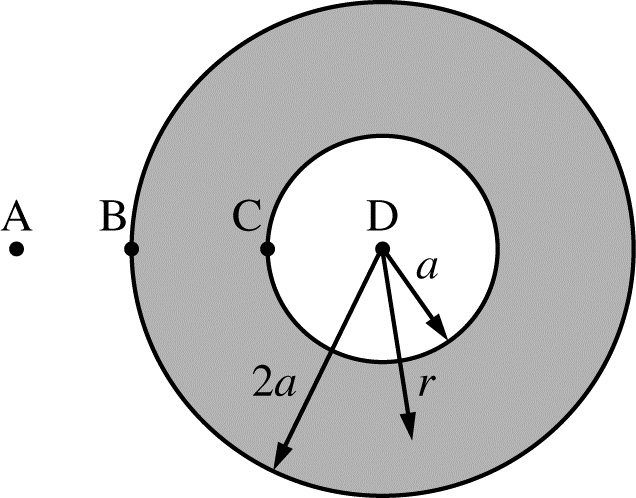
\includegraphics[scale=0.3]{images/img-022-034.png}
\end{figure}


\question
A spherical insulating shell of radius $2 a$ has a hollow cavity of radius $a$, as shown in the figure above. The charge density in the shell for $a<r<2 a$ varies according to the expression $\rho=b r^{2}$, where $b$ is a positive constant and $r$ is the distance from the center of the shell. Express all algebraic answers to the following in terms of $a, b, r$, and fundamental constants, as appropriate. % 请删除并替换本行,与上一行 \question 之间不要留空行

\begin{parts}

%-------------------------------------------------------------------------------
% 请勿删除本注释
% Part (a)
%
% 指引:
% 如在小问之前有通用问题描述,请放置于此
%-------------------------------------------------------------------------------

\part
Derive an expression for the total charge on the shell. % 请删除并替换本行,与上一行 \part 之间不要留空行

%-------------------------------------------------------------------------------
% 请勿删除本注释
% Part (b)
%
% 指引:
% 如在小问之前有通用问题描述,请放置于此
%-------------------------------------------------------------------------------

\part
Using Gauss's law, derive an expression for the magnitude of the electric field in each of the following regions. % 请删除并替换本行,与上一行 \part 之间不要留空行
\begin{subparts}
\subpart $r>2 a$
\subpart $r<a$
\end{subparts}

%-------------------------------------------------------------------------------
% 请勿删除本注释
% Part (c)
%
% 指引:
% 如在小问之前有通用问题描述,请放置于此
%-------------------------------------------------------------------------------

\part
Derive an expression for the electric potential at the outer surface of the shell, where $r=2 a$. Assume the potential to be zero at $r=\infty$. % 请删除并替换本行,与上一行 \part 之间不要留空行

%-------------------------------------------------------------------------------
% 请勿删除本注释
% Part (d)
%
% 指引:
% 如在小问之前有通用问题描述,请放置于此
%-------------------------------------------------------------------------------

\part
Consider the four points $\mathrm{A}, \mathrm{B}, \mathrm{C}$, and $\mathrm{D}$ labeled in the diagram. Rank the four points from highest to lowest based on the electric potential at each point (highest $=1$ ). If two points have the same electric potential, give them the same ranking. % 请删除并替换本行,与上一行 \part 之间不要留空行

\underline{\qquad} A   \quad  \underline{\qquad} B \quad  \underline{\qquad} C  \quad \underline{\qquad} D

Justify your rankings.


\end{parts}
